The text summarization performance of the proposed model is compared against
the BenSumm~\cite{chowdhury-etal-2021-tfidf-clustering}, LexRank~\cite{Erkan-lexRank-2004} and Sentence
Average Similarity-based Spectral Clustering(SASbSC)-based summarization
method~\cite{roychowdhury-etal-2022-spectral-base} methods.
These methods are the recently published state of the art model for Bengali Extractive Text Summarization.
A classic extractive text summarizing method LexRank~\cite{Erkan-lexRank-2004} was also used as a benchmark for comparison.

\subsection{Evaluation Datasets}\label{subsec:evaluation-datasets}
To examine our proposed model, we compared our model along with the 3 benchmark models on 4 different diverse datasets.
We did this so that the results doesn't become biased due to any problem with the dataset.

\subsubsection{Dataset-1 (Self-curated)}
To evaluate the performance of implemented text summarization
methods~\cite{chowdhury-etal-2021-tfidf-clustering,Erkan-lexRank-2004,roychowdhury-etal-2022-spectral-base},
a curated Bengali extractive text summarization dataset was produced by an expert linguistic team.
250 news documents of various sizes were summarized for this purpose.
Each document was summarized twice by two different person to minimize human bias.
In total, there is 500 different document-summary pair in this dataset.
This dataset is made publicly available\footnote{\textit{dataset link}} for other researchers to use for evaluation
purpose in their research.

\subsubsection{Dataset-2 (Towhid Ahmed Foysal)}
This dataset is a collection of summary article pair from The Daily Prothom Alo.
It was published by Towhid Ahmed Foysal in
Kaggle\footnote{\textit{https://www.kaggle.com/datasets/towhidahmedfoysal/bangla-summarization-datasetprothom-alo}}.
The original dataset was filtered so that all the articles smaller than 50 characters and all the summaries
that contains something not in the original articles were discarded.
After filtering, total 10,204 articles remained, each with 2 summaries.

\subsubsection{Dataset-3 (BNLPC)}
This dataset is a collection of news article summaries published by \citeauthor{Hque-2015-BNLPC-Dataset}~\cite{Hque-2015-BNLPC-Dataset}.
The dataset was collected from
GitHub\footnote{\textit{https://github.com/tafseer-nayeem/BengaliSummarization/tree/main/Dataset/BNLPC/Dataset2}}.
The dataset contains 100 article with 3 different summaries for each article.

\subsubsection{Dataset-4 (Abid Mahdi)}
This dataset was published by Abid Mahdi on
GitHub\footnote{\textit{https://github.com/Abid-Mahadi/Bangla-Text-summarization-Dataset}}.
The dataset contains 200 documents each with 2 summaries.

\subsection{Text Summarization Models}\label{subsec:text-summarization-models}
Four different Bengali extractive text summarization models were implemented to evaluate them by
comparing the machine generated summaries against the human generated summaries from the datasets described above.\\

\textbf{Model-1:} Model-1 is the proposed model for this paper.
The model uses word vector based Gaussian similarity to perform spectral clustering to group similar
sentences together and extract one sentence from each group.
This is described as Word Similarity based Spectral Clustering (WSbSC)\\

\textbf{Model-2:} Model-2 (SASbSC) is the method proposed by \citeauthor{roychowdhury-etal-2022-spectral-base}
\cite{roychowdhury-etal-2022-spectral-base}.
This extractive text summarization method is similar to the proposed method.
SCSbSC method uses the same word embedding dataset as ours to get word vectors.
It uses a sentence center similarity based graph to perform spectral clustering inside the method.
Then use cosine similarity to extract sentences from the input.
To get sentence similarity, SCSbSC averages all the word vectors of a particular sentence to get the Sentence center.
This method was implemented in python as described in their article.\\

\textbf{Model-3:} BenSumm describes two different summarization method in the
study~\cite{chowdhury-etal-2021-tfidf-clustering}.
Here only the extractive method is implemented and compared because the proposed method is also extractive in nature.
BenSumm implements a TF-IDF based cosine similarity graph between the sentences and then clusters the sentences using
Agglomerative Clustering.
The implementation codes are publicly available in
GitHub\footnote{\textit{https://github.com/tafseer-nayeem/BengaliSummarization}}.\\

\textbf{Model-4:} LexRank~\cite{Erkan-lexRank-2004} uses a TF-IDF based Matrix and Googles
PageRank algorithm~\cite{page-PageRank-1999} to rank sentences.
The top ranked sentences are selected and arranged into summary after that.
An implemented version of this method is available as a python package in PyPI as
LexRank\footnote{\textit{https://pypi.org/project/lexrank/}}.
LexRank is applied using a large Bengali Wikipedia
corpus\footnote{\textit{https://www.kaggle.com/datasets/shazol/bangla-wikipedia-corpus}}.

\subsection{Evaluation Metrics}\label{subsec:evaluation-metrics}
To evaluate the correctness of the machine generated summaries compared to the human
generated summaries, we used the ROUGE method~\cite{lin-2004-rouge}.
It compares a human produced reference summary with a machine generated summary.
The ROUGE method uses N-gram based overlapping to find a recall, precision and F-1 score.
The ROUGE implementation that were used is available as a python package in
PyPI\footnote{\textit{https://pypi.org/project/rouge/}}.
There are three different metrics in the package for comparison of the summaries.
These are:

\begin{enumerate}
    \item \textbf{ROUGE-1:} It uses unigram matching to find how much similar two summaries are.
    It is a good first impression for performance but can be misleading too as many large enough texts
    will share very high proportion of uni-grams between them.
    \item \textbf{ROUGE-2:} It uses bi-gram matching to find how much similar the two summaries are in a word level.
    Shared bigrams lead to a deeper analysis of syntactic similarities between the two summaries.
    \item \textbf{ROUGE-LCS:} It finds the longest common sub-sequence between the summaries to calculate
    the rouge scores.
    It can calculate the similarity in flow of the sentences between two summaries.
\end{enumerate}

In this study, we compared the F-1 scores from each of these metrics for the 4 models.

\subsection{Comparison}\label{subsec:comparison}
Average F-1 scores for the three Rouge metrics (Rouge-1, Rouge-2, Rouge-LCS) of the four models(Proposed,
SASbSC, BenSumm, LexRank) on the 4 datasets are shown in the table-\ref{tab:result_comparison-1}. \\

\begin{table}[]
    \centering
    \begin{tabular}{lccc} \hline
         Dataset-1 (SC)                                                 &               &               &               \\
         Model                                                          & Rouge-1       & Rouge-2       & Rouge-LCS     \\\hline
         Model-1 (WSbSC)(Proposed)                                      & \textbf{0.47} & \textbf{0.36} & \textbf{0.43} \\
         Model-2 (BenSumm)~\cite{chowdhury-etal-2021-tfidf-clustering}  & 0.41          & 0.29          & 0.36          \\
         Model-3 (SASbSC)~\cite{roychowdhury-etal-2022-spectral-base}   & 0.42          & 0.29          & 0.37          \\
         Model-4 (LexRank)~\cite{Erkan-lexRank-2004}                          & 0.22          & 0.14          & 0.20          \\\hline
         Dataset-2 (TAF)                                                &               &               &               \\\hline
         Model-1 (WSbSC)(Proposed)                                      & \textbf{0.49} & \textbf{0.43} & \textbf{0.48} \\
         Model-2 (BenSumm)~\cite{chowdhury-etal-2021-tfidf-clustering}  & 0.29          & 0.22          & 0.26          \\
         Model-3 (SASbSC)~\cite{roychowdhury-etal-2022-spectral-base}   & 0.23          & 0.12          & 0.18          \\
         Model-4 (LexRank)~\cite{Erkan-lexRank-2004}                          & 0.24          & 0.16          & 0.22          \\\hline
         Dataset-3 (BNLPC)                                              &               &               &               \\\hline
         Model-1 (WSbSC)(Proposed)                                      & \textbf{0.41} & \textbf{0.34} & \textbf{0.40} \\
         Model-2 (BenSumm)~\cite{chowdhury-etal-2021-tfidf-clustering}  & 0.36          & 0.28          & 0.34          \\
         Model-3 (SASbSC)~\cite{roychowdhury-etal-2022-spectral-base}   & \textbf{0.41} & 0.33          & 0.39          \\
         Model-4 (LexRank)~\cite{Erkan-lexRank-2004}                          & 0.26          & 0.19          & 0.24          \\\hline
         Dataset-4 (AM)                                                 &               &               &               \\\hline
         Model-1 (WSbSC)(Proposed)                                      & \textbf{0.49} & \textbf{0.41} & \textbf{0.47} \\
         Model-2 (BenSumm)~\cite{chowdhury-etal-2021-tfidf-clustering}  & 0.31          & 0.22          & 0.28          \\
         Model-3 (SASbSC)~\cite{roychowdhury-etal-2022-spectral-base}   & 0.30          & 0.18          & 0.24          \\
         Model-4 (LexRank)~\cite{Erkan-lexRank-2004}                          & 0.22          & 0.14          & 0.20          \\
    \end{tabular}
    \caption{Comparison of average Rouge scores between graph based extractive summarization models on 4 different datasets}
    \label{tab:result_comparison-1}
\end{table}

These results are further summarized into 3 radar charts so that the performance of each model on each
metric for the datasets can be visualized.

\begin{figure}
    \centering
    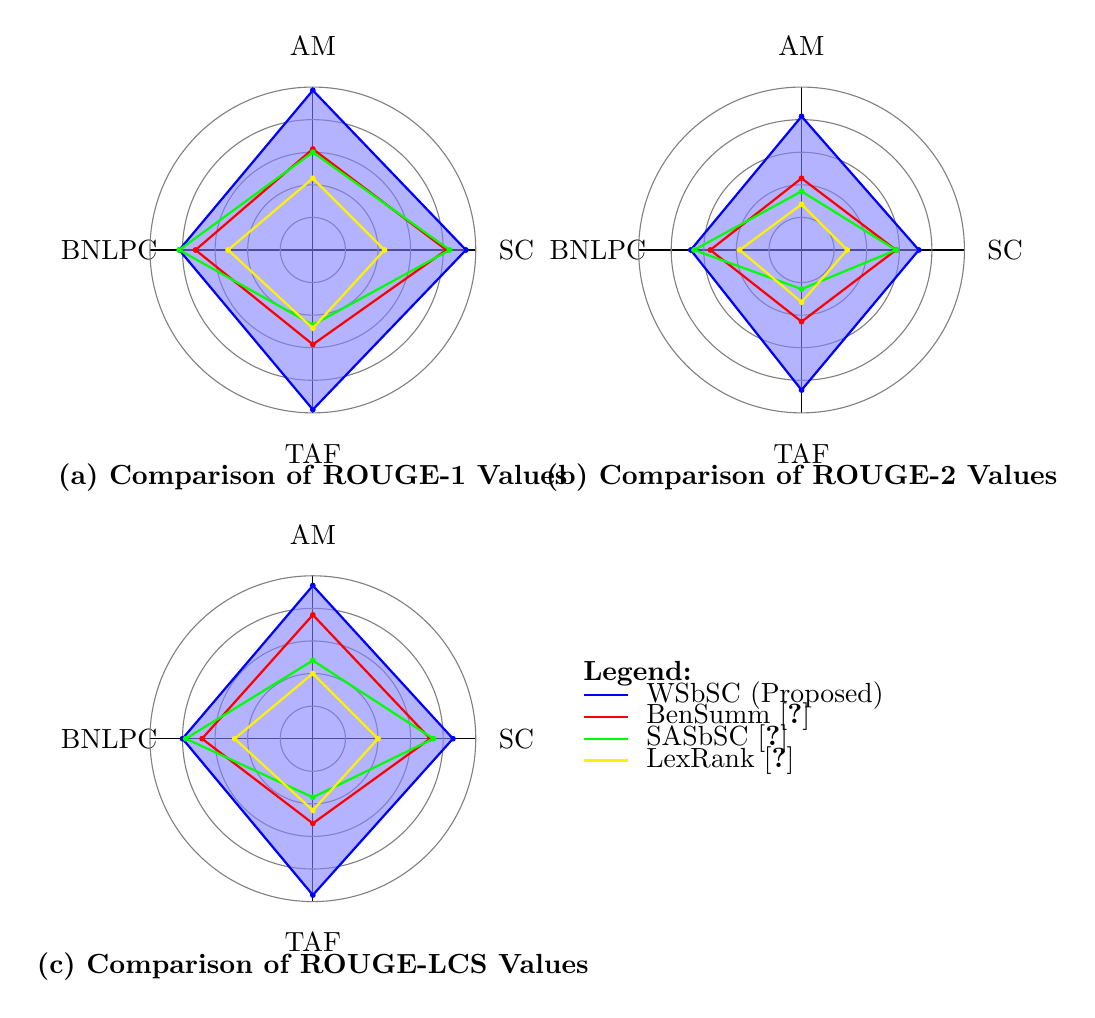
\begin{tikzpicture}[scale=0.002*\textwidth]
    % Define the number of axes (dimensions)
    \def\n{4}
    % Define the names of the features
    \def\features{{"SC", "TAF", "BNLPC", "AM"}}
    % Define the maximum value
    \def\maxvalue{5}

    % Define values for three different radar charts
    \def\valuesAW{{4.7, 4.9, 4.1, 4.9}}
    \def\valuesAB{{4.1, 2.9, 3.6, 3.1}}
    \def\valuesAS{{4.2, 2.3, 4.1, 3.0}}
    \def\valuesAL{{2.2, 2.4, 2.6, 2.2}}

    \def\valuesBW{{3.6, 4.3, 3.4, 4.1}}
    \def\valuesBB{{2.9, 2.2, 2.8, 2.2}}
    \def\valuesBS{{2.9, 1.2, 3.3, 1.8}}
    \def\valuesBL{{1.4, 1.6, 1.9, 1.4}}

    \def\valuesCW{{4.3, 4.8, 4.0, 4.7}}
    \def\valuesCB{{3.6, 2.6, 3.4, 3.8}}
    \def\valuesCS{{3.7, 1.8, 3.9, 2.4}}
    \def\valuesCL{{2.0, 2.2, 2.4, 2.0}}

    % First Radar Chart (Top-left quarter)
    \begin{scope}[xshift=-5cm, yshift=5cm, scale=0.6]
        %write the dataset labels
        \foreach \i in {1,...,\n} {
            \draw (90-\i*360/\n:5) -- (0,0);
            \node at (90-\i*360/\n:6.25) {\pgfmathparse{\features[\i-1]}\pgfmathresult};
        }
        %draw the circle
        \node at (90-2*360/4:7){\textbf{(a) Comparison of ROUGE-1 Values}};
        \foreach \j in {1,...,\maxvalue} {
            \draw[gray, thin] (0,0) circle (\j);
        }

        %draw wsbsc
        \foreach \i [evaluate={\angle=90-\i*360/\n; \valueAW=\valuesAW[\i-1];}] in {1,...,\n} {
            \coordinate (PA\i) at (\angle:\valueAW);
            \filldraw[blue] (PA\i) circle (2pt);
        }
        \fill[blue!50, opacity=0.6] (PA1) -- (PA2) -- (PA3) -- (PA4) -- cycle;
        \foreach \i in {1,...,\n} {
            \pgfmathtruncatemacro{\nexti}{mod(\i,\n)+1}
%                    \draw [thick, cyan] plot [smooth, tension=2] coordinates { (PA\i) (PA\nexti)};
            \draw[thick, blue] (PA\i) -- (PA\nexti);
        }
%                \draw [thick,cyan] plot [smooth cycle, tension=1] coordinates { (PA1) (PA2) (PA3) (PA4)};

        %draw bensumm
        \foreach \i [evaluate={\angle=90-\i*360/\n; \valueAB=\valuesAB[\i-1];}] in {1,...,\n} {
            \coordinate (PB\i) at (\angle:\valueAB);
            \filldraw[red] (PB\i) circle (2pt);
        }
        \foreach \i in {1,...,\n} {
            \pgfmathtruncatemacro{\nexti}{mod(\i,\n)+1}
            \draw[thick, red] (PB\i) -- (PB\nexti);
        }

%                draw sasbsc
        \foreach \i [evaluate={\angle=90-\i*360/\n; \valueAS=\valuesAS[\i-1];}] in {1,...,\n} {
            \coordinate (PC\i) at (\angle:\valueAS);
            \filldraw[green] (PC\i) circle (2pt);
        }
        \foreach \i in {1,...,\n} {
            \pgfmathtruncatemacro{\nexti}{mod(\i,\n)+1}
            \draw[thick, green] (PC\i) -- (PC\nexti);
        }

        %draw lexrank
        \foreach \i [evaluate={\angle=90-\i*360/\n; \valueAL=\valuesAL[\i-1];}] in {1,...,\n} {
            \coordinate (PD\i) at (\angle:\valueAL);
            \filldraw[yellow] (PD\i) circle (2pt);
        }
        \foreach \i in {1,...,\n} {
            \pgfmathtruncatemacro{\nexti}{mod(\i,\n)+1}
            \draw[thick, yellow] (PD\i) -- (PD\nexti);
        }
    \end{scope}

    % Second Radar Chart (Top-right quarter)
    \begin{scope}[xshift=4cm, yshift=5cm, scale=0.6]
        \foreach \i in {1,...,\n} {
            \draw (90-\i*360/\n:5) -- (0,0);
            \node at (90-\i*360/\n:6.25) {\pgfmathparse{\features[\i-1]}\pgfmathresult};
        }
        \node at (90-2*360/4:7){\textbf{(b) Comparison of ROUGE-2 Values}};
        \foreach \j in {1,...,\maxvalue} {
            \draw[gray, thin] (0,0) circle (\j);
        }

        \foreach \i [evaluate={\angle=90-\i*360/\n; \valueBW=\valuesBW[\i-1];}] in {1,...,\n} {
            \coordinate (PA\i) at (\angle:\valueBW);
            \filldraw[blue] (PA\i) circle (2pt);
        }
        \fill[blue!50, opacity=0.6] (PA1) -- (PA2) -- (PA3) -- (PA4) -- cycle;
        \foreach \i in {1,...,\n} {
            \pgfmathtruncatemacro{\nexti}{mod(\i,\n)+1}
            \draw[thick, blue] (PA\i) -- (PA\nexti);
        }

        \foreach \i [evaluate={\angle=90-\i*360/\n; \valueBB=\valuesBB[\i-1];}] in {1,...,\n} {
            \coordinate (PB\i) at (\angle:\valueBB);
            \filldraw[red] (PB\i) circle (2pt);
        }
        \foreach \i in {1,...,\n} {
            \pgfmathtruncatemacro{\nexti}{mod(\i,\n)+1}
            \draw[thick, red] (PB\i) -- (PB\nexti);
        }

        \foreach \i [evaluate={\angle=90-\i*360/\n; \valueBS=\valuesBS[\i-1];}] in {1,...,\n} {
            \coordinate (PC\i) at (\angle:\valueBS);
            \filldraw[green] (PC\i) circle (2pt);
        }
        \foreach \i in {1,...,\n} {
            \pgfmathtruncatemacro{\nexti}{mod(\i,\n)+1}
            \draw[thick, green] (PC\i) -- (PC\nexti);
        }

        \foreach \i [evaluate={\angle=90-\i*360/\n; \valueBL=\valuesBL[\i-1];}] in {1,...,\n} {
            \coordinate (PD\i) at (\angle:\valueBL);
            \filldraw[yellow] (PD\i) circle (2pt);
        }
        \foreach \i in {1,...,\n} {
            \pgfmathtruncatemacro{\nexti}{mod(\i,\n)+1}
            \draw[thick, yellow] (PD\i) -- (PD\nexti);
        }
    \end{scope}

    % Third Radar Chart (Bottom-left quarter)
    \begin{scope}[xshift=-5cm, yshift=-4cm, scale=0.6]
        \foreach \i in {1,...,\n} {
            \draw (90-\i*360/\n:5) -- (0,0);
            \node at (90-\i*360/\n:6.25) {\pgfmathparse{\features[\i-1]}\pgfmathresult};
        }
        \node at (90-2*360/4:7){\textbf{(c) Comparison of ROUGE-LCS Values}};
        \foreach \j in {1,...,\maxvalue} {
            \draw[gray, thin] (0,0) circle (\j);
        }

        \foreach \i [evaluate={\angle=90-\i*360/\n; \valueCW=\valuesCW[\i-1];}] in {1,...,\n} {
            \coordinate (PA\i) at (\angle:\valueCW);
            \filldraw[blue] (PA\i) circle (2pt);
        }
        \fill[blue!50, opacity=0.6] (PA1) -- (PA2) -- (PA3) -- (PA4) -- cycle;
        \foreach \i in {1,...,\n} {
            \pgfmathtruncatemacro{\nexti}{mod(\i,\n)+1}
            \draw[thick, blue] (PA\i) -- (PA\nexti);
        }

        \foreach \i [evaluate={\angle=90-\i*360/\n; \valueCB=\valuesCB[\i-1];}] in {1,...,\n} {
            \coordinate (PB\i) at (\angle:\valueCB);
            \filldraw[red] (PB\i) circle (2pt);
        }
        \foreach \i in {1,...,\n} {
            \pgfmathtruncatemacro{\nexti}{mod(\i,\n)+1}
            \draw[thick, red] (PB\i) -- (PB\nexti);
        }

        \foreach \i [evaluate={\angle=90-\i*360/\n; \valueCS=\valuesCS[\i-1];}] in {1,...,\n} {
            \coordinate (PC\i) at (\angle:\valueCS);
            \filldraw[green] (PC\i) circle (2pt);
        }
        \foreach \i in {1,...,\n} {
            \pgfmathtruncatemacro{\nexti}{mod(\i,\n)+1}
            \draw[thick, green] (PC\i) -- (PC\nexti);
        }

        \foreach \i [evaluate={\angle=90-\i*360/\n; \valueCL=\valuesCL[\i-1];}] in {1,...,\n} {
            \coordinate (PD\i) at (\angle:\valueCL);
            \filldraw[yellow] (PD\i) circle (2pt);
        }
        \foreach \i in {1,...,\n} {
            \pgfmathtruncatemacro{\nexti}{mod(\i,\n)+1}
            \draw[thick, yellow] (PD\i) -- (PD\nexti);
        }
    \end{scope}

    % Legend (Bottom-right quarter)
    \begin{scope}[xshift=4cm, yshift=-4cm, scale=0.8]
        \node[anchor=west] at (-5.25, 1.5) {\textbf{Legend:}};
        \draw[thick, blue] (-5, 1) -- (-4, 1);
        \node[anchor=west] at (-3.8, 1) {WSbSC (Proposed)};

        \draw[thick, red] (-5, 0.5) -- (-4, 0.5);
        \node[anchor=west] at (-3.8, 0.5) {BenSumm~\cite{chowdhury-etal-2021-tfidf-clustering}};

        \draw[thick, green] (-5, 0) -- (-4, 0);
        \node[anchor=west] at (-3.8, 0) {SASbSC~\cite{roychowdhury-etal-2022-spectral-base}};

        \draw[thick, yellow] (-5, -0.5) -- (-4, -0.5);
        \node[anchor=west] at (-3.8, -0.5) {LexRank~\cite{Erkan-lexRank-2004}};
    \end{scope}
\end{tikzpicture}
    \caption{Radar chart of the models being compared on 3 different metrics and 4 datasets.}
    \label{fig:radarchart}
 \end{figure}

These charts (Figure~\ref{fig:radarchart}) shows us that the proposed method is much more dataset independent and performs
uniformly on every metric across the datasets.
Other models although performs good on certain datasets, fails to show consistency.

\subsection{Different Ranking Techniques Inside Clusters}\label{subsec:different-ranking-techniques-inside-clusters}
We implemented two ranking methods to pick the best sentence from each clusters.
First one is the First Rank method where we just pick the sentence that is first in terms of their order of
appearance inside the input document.
The second one is the TF-IDF ranking, where we ranked the sentences by their TF-IDF scores and pick the best one.
We can see in the table~\ref{tab:ranking} that the TF-IDF scores better on a high quality dataset like our Self-curated one.

\begin{table}\label{tab:ranking}
    \centering
    \begin{tabular}{cccc}\hline
        Method      & Rouge-1       & Rouge-2       & Rouge-LCS     \\\hline
        FirstRank   & 0.47          & 0.36          & 0.43          \\
        TF-IDF      & \textbf{0.50} & \textbf{0.40} & \textbf{0.46} \\\hline
    \end{tabular}
    \caption{Comparison of Result of different ranking techniques}
\end{table}

\subsection{Implementation Into Other Languages}\label{subsec:implementation-into-other-languages}
The model discussed here is not language dependent.
So the model can be easily extended into other languages.
To perform this method into a language, we only need a language specific tokenizer, a list of stop-words and
a word vector embedding dataset.
We tried to find quality extractive text summarization dataset for evaluating the method, but could only
find relevant datasets on 3 other languages.
These are Hindi, Marathi and Turkish.
We adopted this Model into these 3 low resource languages to check this hypothesis.\\

\begin{table}
    \centering
    \begin{tabular}{cccc}\hline
        Language                & Rouge-1   & Rouge-2   & Rouge-LCS \\\hline
        Bengali (Dataset - 1)   & 0.47      & 0.36      & 0.43      \\
        Bengali (Dataset - 2)   & 0.49      & 0.43      & 0.48      \\
        Bengali (Dataset - 3)   & 0.41      & 0.34      & 0.40      \\
        Bengali (Dataset - 4)   & 0.49      & 0.41      & 0.47      \\
        Bengali (Average)       & 0.47      & 0.38      & 0.44      \\\hline
        Hindi                   & 0.40      & 0.26      & 0.36      \\\hline
        Marathi                 & 0.50	    & 0.42      & 0.50      \\\hline
        Turkish                 & 0.48      & 0.39      & 0.47      \\\hline
    \end{tabular}
    \caption{Comparison of Result of proposed summarization method in other low-resource languages}
    \label{tab:other_language}
\end{table}

The Table-\ref{tab:other_language} shows the result of the proposed word similarity based spectral clustering
method for extractive summarization in other low resource languages.
For the Hindi language, we used a Kaggle
dataset\footnote{\textit{https://www.kaggle.com/datasets/disisbig/hindi-text-short-and-large-summarization-corpus/}}
produced by Gaurav Arora.
For the Marathi language we used another Kaggle
dataset\footnote{\textit{https://www.kaggle.com/datasets/ketki19/marathi}} produced by Ketki Nirantar.
For the Turkish language we used a Github
dataset\footnote{\textit{https://github.com/xtinge/turkish-extractive-summarization-dataset/blob/main/dataset/XTINGE-SUM\_TR\_EXT/xtinge-sum\_tr\_ext.json}}
produced by the XTINGE~\cite{Demir-2024-xtinge_turkish_extractive} team.
We can see that the results remain very close despite the change in language.


